\section{Schrödinger problem for Landau levels in dressed 2DEG}

Our analysis start with considering 2 dimentional free electronic gas which has been distrubuted in confined $(x,y)$ plane in configuration space.
\begin{figure}[ht!]
  \centering
  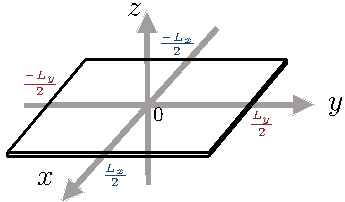
\includegraphics[scale=0.9]{figures/fig0.pdf}
  \caption{Confined 2DEG in configuration space with the size of $A=L_xL_y$.}
  \label{fig:1.0}
\end{figure}

\noindent
We are going to examine the properties of 2DEG with stationary magnetic field
\begin{equation} \label{1.1}
  \vb{B} = (0,0,B)^T
\end{equation}
which directed on $z$ axis and a linearly $y$-polarized strong electomagnetic wave (dressing field) with electric field given by
\begin{equation} \label{1.2}
  \vb{E} = (0,E\sin(\omega t),0)^T
\end{equation}
which also propagate in $z$ direction. Here $B$ and $E$ represent the amplitude of the stationary magnetic field and electric field of dressing field.
\begin{figure}[ht!]
  \centering
  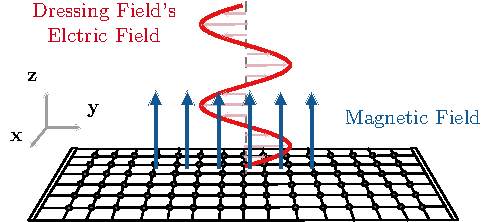
\includegraphics[scale=0.9]{figures/fig1.pdf}
  \caption{Stationary magnetic filed (blue color) and Strong EM wave (red color) applied to the 2DEG.}
  \label{fig:1.1}
\end{figure}

\noindent
Using Landau gauge for the stationary magnetic field we can represent it using vector potential as
\begin{equation} \label{1.3}
  \vb{A}_{s} = (-By,0,0)^T
\end{equation}
and choosing Coulomb gauge the dressing field can be present as the following vector potential
\begin{equation} \label{1.4}
  \vb{A}_{d}(t) = (0,[E/\omega ]\cos(\omega t),0)^T.
\end{equation}
Now the Hamiltonian of an electron in 2DEG can be reads as
\begin{equation} \label{1.5}
  \hat{H}_e(t) = \frac{1}{2m_e}\Big[\hat{\vb{p}} - e\big(\vb{A}_{s}+\vb{A}_{d}(t)\big)\Big]^2
\end{equation}
where $m_e$ is the effective mass of the electron and $e$ is the magnitude (without considering the sign of the charge) of the electron charge. This can be simplified to
\begin{equation} \label{1.6}
  \hat{H}_e(t) = \frac{1}{2m_e}\Big[
    (\hat{p}_x + eBy)\vb{e}_x +
    (\hat{p}_y - \frac{eE}{\omega}\cos(\omega t))\vb{e}_y
  \Big]^2
\end{equation}
where $\vb{e}_x$ and $\vb{e}_y$ are unit vectors along $x$ and $y$ directions respectively. Moreover,
\begin{equation} \label{1.7}
  \hat{H}_e(t) = \frac{1}{2m_e}\Big[
    (\hat{p}_x + eBy)^2 +
    (\hat{p}_y - \frac{eE}{\omega}\cos(\omega t))^2
  \Big]
\end{equation}
Since $[\hat{H}_e(t),\hat{p}_x] =0$ both operators share same (simultaneous) eigen functions which are free electron wave functions
($\frac{1}{\sqrt{L_x}}\exp(\frac{ip_x x}{\hbar})$).
Therefore we can modify the Hamiltonian as follows
\begin{equation} \label{1.8}
  \hat{H}_e(t) = \frac{1}{2m_e}\Big[
    ({p}_x + eBy)^2 +
    (\hat{p}_y - \frac{eE}{\omega}\cos(\omega t))^2
  \Big].
\end{equation}
Using momentum operator definition
\begin{equation} \label{1.9}
  \hat{p}_y = -i\hbar \pdv{y}
\end{equation}
we can modify Eq. \eqref{1.8} as
\begin{equation} \label{1.10}
  \begin{aligned}
    \hat{H}_e(t) & = \frac{1}{2m_e}\Big[
      ({p}_x + eBy)^2 +
      \Big(-i\hbar \pdv{y}- \frac{eE}{\omega}\cos(\omega t)\Big)^2
    \Big] \\
    & = \frac{1}{2m_e}\Big[
      ({p}_x + eBy)^2 +
      \Big(i\hbar \pdv{y} + \frac{eE}{\omega}\cos(\omega t)\Big)^2
    \Big].
  \end{aligned}
\end{equation}
Define the \textit{center of the cyclotron orbit} along $y$ axis as
\begin{equation} \label{1.11}
  y_0 \equiv \frac{-p_x}{eB}
\end{equation}
and the \textit{cyclotron frequency} as
\begin{equation} \label{1.12}
  \omega_0 \equiv \frac{eB}{m_e}.
\end{equation}
\begin{figure}[ht!]
  \centering
  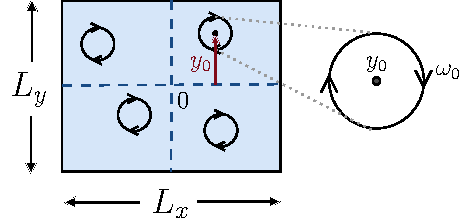
\includegraphics[scale=0.9]{figures/fig02.pdf}
  \caption{Paramters of the cyclotron orbits in the classical interpretation.}
  \label{fig:1.02}
\end{figure}

\noindent
Then the Hamiltonian will leads to
\begin{equation} \label{1.13}
    \hat{H}_e(t) =
      \frac{m_e \omega_0^2}{2}(y-y_0)^2 +
      \frac{1}{2m_e}\Big(i\hbar \pdv{y}+\frac{eE}{\omega}\cos(\omega t)\Big)^2
\end{equation}
\begin{equation} \label{1.14}
  \begin{aligned}
    \hat{H}_e(t) =
      \frac{m_e \omega_0^2}{2}(y-y_0)^2 +
      \frac{1}{2m_e}\Big(
      -\hbar^2 \pdv[2]{y} & +
      i\hbar \pdv{y}\bigg[\frac{eE}{\omega}\cos(\omega t) \bigg] \\ & +
      \frac{i\hbar eE}{\omega}\cos(\omega t) \pdv{y}+
      \frac{e^2E^2}{\omega^2}\cos[2](\omega t)
      \Big)
  \end{aligned}
\end{equation}
\begin{equation} \label{1.15}
  \begin{aligned}
    \hat{H}_e(t) =
      \frac{m_e \omega_0^2}{2}(y-y_0)^2 +
      \frac{1}{2m_e}\Big(
      -\hbar^2 \pdv[2]{y} +
      \frac{2i\hbar eE}{\omega}\cos(\omega t) \pdv{y}+
      \frac{e^2E^2}{\omega^2}\cos[2](\omega t)
      \Big).
  \end{aligned}
\end{equation}
Let
\begin{equation} \label{1.16}
    \tilde{y} = (y - y_0) \longrightarrow dy = d\tilde{y}
\end{equation}
and then this becomes
\begin{equation} \label{1.17}
  \begin{aligned}
    \hat{H}_e(t) =
      \frac{m_e \omega_0^2}{2}\tilde{y}^2 +
      \frac{1}{2m_e}\Big(
      -\hbar^2 \pdv[2]{\tilde{y}} +
      \frac{2i\hbar eE}{\omega}\cos(\omega t) \pdv{\tilde{y}}+
      \frac{e^2E^2}{\omega^2}\cos[2](\omega t)
      \Big).
  \end{aligned}
\end{equation}
Now assume that the solution for the time-dependent schrödinger equation
\begin{equation} \label{1.18}
    i \hbar \dv{\psi}{t} = \hat{H}_e(t)\psi
\end{equation}
can be represent by the following form
\begin{equation} \label{1.19}
    \psi(\vb{r},t) = \frac{1}{\sqrt{L_x}} \exp\bigg(
      \frac{ip_x x}{\hbar} +
      \frac{ieE(y-y_0)}{\hbar \omega}\cos(\omega t)
    \bigg) \phi(y-y_0,t).
\end{equation}
Using the same subtution from Eq. \eqref{1.16} this becomes
\begin{equation} \label{1.20}
    \psi(x,\tilde{y},t) = \frac{1}{\sqrt{L_x}} \exp\bigg(
      \frac{ip_x x}{\hbar} +
      \frac{ieE\tilde{y}}{\hbar \omega}\cos(\omega t)
    \bigg) \phi(\tilde{y},t).
\end{equation}
Defining
\begin{equation} \label{1.21}
    \varphi(x,\tilde{y},t) \equiv \frac{1}{\sqrt{L_x}} \exp\bigg(
      \frac{ip_x x}{\hbar} +
      \frac{ieE\tilde{y}}{\hbar \omega}\cos(\omega t)
    \bigg)
\end{equation}
we can simply the the Eq. \eqref{1.20} as
\begin{equation} \label{1.22}
    \psi(x,\tilde{y},t) = \varphi(x,\tilde{y},t) \phi(\tilde{y},t).
\end{equation}
Let's subtitue Eq. \eqref{1.20} and Eq. \eqref{1.17} into Eq. \eqref{1.18} and we can observe that
\begin{equation} \label{1.23}
  \begin{aligned}
    \text{L.H.S} & = i \hbar \dv{\psi}{t} =
    i \hbar \bigg( \dv{\varphi}{t} \phi + \dv{\phi}{t} \varphi \bigg) =
    i \hbar \bigg(
      \Big[\frac{-ieE\tilde{y}}{\hbar}\sin(\omega t)\Big]\varphi\phi +
      \varphi  \dv{\phi}{t}
    \bigg) \\
    & =
    \big[{eE\tilde{y}}\sin(\omega t)\big]\varphi\phi +
    i \hbar\varphi  \dv{\phi}{t}
  \end{aligned}
\end{equation}
and
\begin{equation} \label{1.24}
  \begin{aligned}
    \text{R.H.S} & = \hat{H}_e(t)\psi \\
    & =
    \bigg[
    \frac{m_e \omega_0^2}{2}\tilde{y}^2 +
    \frac{1}{2m_e}\Big(
    -\hbar^2 \pdv[2]{\tilde{y}} +
    \frac{2i\hbar eE}{\omega}\cos(\omega t) \pdv{\tilde{y}}+
    \frac{e^2E^2}{\omega^2}\cos[2](\omega t)
    \Big) \bigg]
    \varphi\phi
  \end{aligned}
\end{equation}
where we will can calculate this part by part as follows:
\begin{equation} \label{1.25}
  \begin{aligned}
    \frac{-\hbar^2}{2m_e}\pdv[2]{\tilde{y}}(\varphi\phi) & =
    \frac{-\hbar^2}{2m_e} \pdv{\tilde{y}}\bigg[
      \Big(\frac{ieE}{\hbar \omega} \cos(\omega)t\Big)\varphi\phi +
      \varphi\pdv{\phi}{\tilde{y}}
    \bigg] \\
    & =
    \frac{-\hbar^2}{2m_e} \bigg[
      \Big(\frac{ieE}{\hbar \omega} \cos(\omega)t\Big)^2\varphi\phi +
      \Big(\frac{ieE}{\hbar \omega} \cos(\omega)t\Big)\varphi\pdv{\phi}{\tilde{y}} +
      \Big(\frac{ieE}{\hbar \omega} \cos(\omega)t\Big)\varphi\pdv{\phi}{\tilde{y}} +
      \varphi\pdv[2]{\phi}{\tilde{y}}
    \bigg] \\
    & =
    \Big(\frac{e^2E^2}{ 2m_e\omega^2} \cos[2](\omega)t\Big)\varphi\phi -
    \Big(\frac{ieE \hbar}{m_e\omega} \cos(\omega)t\Big)\varphi\pdv{\phi}{\tilde{y}} -
    \frac{\hbar^2}{2m_e}
    \varphi\pdv[2]{\phi}{\tilde{y}}
  \end{aligned}
\end{equation}
and
\begin{equation} \label{1.26}
  \begin{aligned}
    \frac{2i\hbar eE}{2m_e\omega}\cos(\omega t) \pdv{\tilde{y}} (\varphi\phi)& =
    \frac{i\hbar eE}{m_e\omega}\cos(\omega t)
    \bigg[
      \Big(\frac{ieE}{\hbar \omega} \cos(\omega)t\Big)\varphi\phi +
      \varphi\pdv{\phi}{\tilde{y}}
    \bigg] \\
    & =
    \Big(\frac{-e^2E^2}{m_e\omega^2} \cos(\omega)t\Big)\varphi\phi +
    \frac{i\hbar eE}{m_e\omega}\cos(\omega t)\varphi\pdv{\phi}{\tilde{y}}.
  \end{aligned}
\end{equation}
Therefore we can derive that
\begin{equation} \label{1.27}
  \begin{aligned}
    \text{R.H.S} =
    \bigg[
    \frac{m_e \omega_0^2}{2}\tilde{y}^2 \varphi\phi
    -
    \frac{\hbar^2}{2m_e}
    \varphi\pdv[2]{\phi}{\tilde{y}} \bigg].
  \end{aligned}
\end{equation}
To satisfy the condition L.H.S$=$R.H.S we need to find a function $\phi(\tilde{y},t)$ such that
\begin{equation} \label{1.28}
  \begin{aligned}
    \big[{eE\tilde{y}}\sin(\omega t)\big]\varphi\phi +
    i \hbar\varphi  \dv{\phi}{t}
    =
    \bigg[
    \frac{m_e \omega_0^2}{2}\tilde{y}^2 \varphi\phi
    -
    \frac{\hbar^2}{2m_e}
    \varphi\pdv[2]{\phi}{\tilde{y}} \bigg]
  \end{aligned}
\end{equation}
by removing $\varphi$ this can be simplyfied as
\begin{equation} \label{1.29}
  \begin{aligned}
    \bigg[
    \frac{m_e \omega_0^2}{2}\tilde{y}^2
    - {eE\tilde{y}}\sin(\omega t)
    -
    \frac{\hbar^2}{2m_e}
    \pdv[2]{\tilde{y}}
    - i \hbar \dv{t}
    \bigg]
    \phi(\tilde{y},t) = 0.
  \end{aligned}
\end{equation}
If we turn off the external dressing field, this equation leads to simple harmonic oscillator Hamiltonian as follows
\begin{equation} \label{1.30}
  \begin{aligned}
    \bigg[
    \frac{m_e \omega_0^2}{2}\tilde{y}^2
    -
    \frac{\hbar^2}{2m_e}
    \pdv[2]{\tilde{y}}
    - i \hbar \dv{t}
    \bigg]
    \phi(\tilde{y},t) = 0
  \end{aligned}
\end{equation}
\begin{equation} \label{1.31}
  \begin{aligned}
     i \hbar \dv{\phi(\tilde{y},t)}{t} =
    \bigg[
    \frac{\hat{p}_{\tilde{y}}^2}{2m_e} +
    \frac{1}{2}m_e \omega_0^2\tilde{y}^2
    \bigg]
    \phi(\tilde{y},t).
  \end{aligned}
\end{equation}
Therefore we can identify the $S(t) \equiv eE\sin(\omega t)$ part as a external force act on the harmonic oscillator and we can solve this as a forced harmonic oscillator in $\tilde{y}$ axis.
\begin{equation} \label{1.32}
  \begin{aligned}
    i \hbar \dv{\phi(\tilde{y},t)}{t} =
    \bigg[
    -
    \frac{\hbar^2}{2m_e}
    \pdv[2]{\tilde{y}} +
    \frac{1}{2}m_e \omega_0^2\tilde{y}^2
    - \tilde{y}S(t)]
    \bigg]
    \phi(\tilde{y},t).
  \end{aligned}
\end{equation}
This system can be extacly solvable and we can solve this equation using the methods explained by Husimi [*Ref:1] as follows.

\noindent
First we can introduce the time dependent shifted corrdinte as
\begin{equation} \label{1.33}
    \tilde{y} \rightarrow y' = \tilde{y} - \zeta(t) \quad \Rightarrow \quad
    \tilde{y} = y' + \zeta(t)
\end{equation}
and this implies that
\begin{equation} \label{1.34}
    \dv{\phi(y',t)}{t} = \pdv{\phi(y',t)}{t} + \pdv{\phi(y',t)}{y'}\pdv{y'}{t} =
    \pdv{\phi(y',t)}{t} - \dot{\zeta}(t)\pdv{\phi(y',t)}{y'}
\end{equation}
where $\dot{\zeta}(t) = \pdv{\zeta(t)}{t}$.
Therefore, Eq. \eqref{1.32} will be modified to
\begin{equation} \label{1.35}
  \begin{aligned}
    i \hbar \pdv{\phi(y',t)}{t}  =
    \bigg[
    i \hbar\dot{\zeta}\pdv{y'}
    -
    \frac{\hbar^2}{2m_e}
    \pdv[2]{{y'}} +
    \frac{1}{2}m_e \omega_0^2(y' + \zeta)^2
    - (y' + \zeta) S(t)
    \bigg]
    \phi(y',t).
  \end{aligned}
\end{equation}
Let's tranform the wave function using following unitary trasnform
\begin{equation} \label{1.36}
    \phi(y',t) = \exp(\frac{im_e\dot{\zeta}y'}{\hbar})\varphi(y',t)
\end{equation}
and subtitte this into the Eq. \eqref{1.35} and we will get the following
\begin{equation} \label{1.37}
  \text{L.H.S} =  \bigg[ i \hbar \pdv{t} -
i \hbar \Big(\frac{im_e \ddot{\zeta} y'}{\hbar}\Big)\bigg]  \exp(\frac{-im_e\dot{\zeta}y'}{\hbar})\varphi(y',t)
\end{equation}
and
\begin{equation} \label{1.38}
  \begin{aligned}
    \text{R.H.S} & =  \bigg[
      i \hbar \dot{\zeta}  \Big(\frac{im_e \dot{\zeta}}{\hbar}\Big)  +
      i \hbar \dot{\zeta} \pdv{y'} \\
      &
      -
      \frac{\hbar^2}{2m_e}\Big[
        \Big(\frac{im_e \dot{\zeta}}{\hbar}\Big)^2
        + \Big(\frac{2im_e \dot{\zeta}}{\hbar}\Big) \pdv{{y'}}
        + \pdv[2]{{y'}}
      \Big] \\
      &
      +\frac{1}{2}m_e\omega_0^2 {y'}^2 + \frac{1}{2}m_e\omega_0^2 \zeta^2 +
      m_e\omega_0^2 y'\zeta \\
      & -
      y'S(t) - \zeta S(t)
    \bigg]  \exp(\frac{-im_e\dot{\zeta}y'}{\hbar})\varphi(y',t).
  \end{aligned}
\end{equation}
Combining these two and removing exponential terms we can derive that
\begin{equation} \label{1.39}
  \begin{aligned}
    i \hbar \pdv{\varphi(y',t)}{t}   =
    \bigg[
        -  \frac{\hbar^2}{2m_e}\pdv[2]{{y'}}
        & + \frac{1}{2} m_e \omega_0^2 y'^2 +
        \Big[
            m_e\ddot{\zeta} + m_e\omega_0^2\zeta - S(t)
        \Big]y' \\
        &
        +
        \Big[
            - \frac{1}{2} m_e\dot{\zeta}^2 + \frac{1}{2}m_e\omega_0^2 \zeta^2 - \zeta S(t)
        \Big]
    \bigg]\varphi(y',t).
  \end{aligned}
\end{equation}
Then we can restrict our $\zeta(t)$ function such that
\begin{equation} \label{1.40}
  m_e\ddot{\zeta} + m_e\omega_0^2\zeta = S(t)
\end{equation}
and that leads to
\begin{equation} \label{1.41}
  \begin{aligned}
    i \hbar \pdv{\varphi(y',t)}{t}   =
    \bigg[
        -  \frac{\hbar^2}{2m_e}\pdv[2]{{y'}}
        + \frac{1}{2} m_e \omega_0^2 {y'}^2
        - L(\zeta,\dot{\zeta},t)
    \bigg]\varphi(y',t)
  \end{aligned}
\end{equation}
where
\begin{equation} \label{1.42}
  L(\zeta,\dot{\zeta},t) \equiv \frac{1}{2} m_e\dot{\zeta}^2 - \frac{1}{2}m_e\omega_0^2 \zeta^2 + \zeta S(t)
\end{equation}
is the largrangian of a classical driven oscillator.

\vspace{5mm}
\noindent
Now introduce new unitary transormation for the wavefunction as follows
\begin{equation} \label{1.43}
    \varphi(y',t) = \exp(\frac{i}{\hbar}\int_0^{t}dt'L(\zeta,\dot{\zeta},t')) \chi(y',t)
\end{equation}
and subtite this into the Eq. \eqref{1.41} and gets
\begin{equation} \label{1.44}
  \begin{aligned}
    i \hbar \bigg[
      & \exp(\frac{i}{\hbar}\int_0^{t}dt'L(\zeta,\dot{\zeta},t')) \pdv{t}
      +
      i \hbar L(\zeta,\dot{\zeta},t) \exp(\frac{i}{\hbar}\int_0^{t}dt'L(\zeta,\dot{\zeta},t'))
    \bigg]\chi(y',t) \\
    & =
    \bigg[
        -  \frac{\hbar^2}{2m_e}\pdv[2]{{y'}}
        + \frac{1}{2} m_e \omega_0^2 {y'}^2
        - L(\zeta,\dot{\zeta},t)
    \bigg] \exp(\frac{i}{\hbar}\int_0^{t}dt'L(\zeta,\dot{\zeta},t')) \chi(y',t)
  \end{aligned}
\end{equation}
removing exponential terms finally we can derive that
\begin{equation} \label{1.45}
  \begin{aligned}
    i \hbar \pdv{t} \chi(y',t)  =
    \bigg[
        -  \frac{\hbar^2}{2m_e}\pdv[2]{{y'}}
        + \frac{1}{2} m_e \omega_0^2 {y'}^2
    \bigg] \chi(y',t).
  \end{aligned}
\end{equation}
This is the well known Schrodinger equation of a stationary quantum harmonic oscillator.
In terms of the eigenvalues
\begin{equation} \label{1.46}
  E_n = \hbar \omega_0 \big(n + \frac{1}{2}\big)
\end{equation}
of well-known harmonic eigenfucntions (Gauss-Hermite functions)
\begin{equation} \label{1.47}
  \chi_n(x) \equiv \frac{\sqrt{\kappa}}{\sqrt{2^{n}n!}}
  e^{-\kappa^2 x^2}
  \mathcal{H}_n \qty(\kappa x) \quad \text{where}
  \quad
  \kappa = \sqrt{\frac{m_e \omega_0}{\hbar}}
\end{equation}
being propositional to the Hermite functions $\mathcal{H}_n$, the solutions of Eq. \eqref{1.32} can be represent as
\begin{equation} \label{1.48}
  \phi_n(\tilde{y},t) = \chi_n(\tilde{y} - \zeta(t))
  \exp(\frac{i}{\hbar}\bigg[- E_nt +
  m_e\dot{\zeta(t)}\big(\tilde{y}-\zeta(t)\big)
   + \int_0^{t}dt'L(\zeta,\dot{\zeta},t')\bigg])
\end{equation}
The set $\{\chi_n(x)\}$ forms a complete set and thus any general solution $\phi_(\tilde{y},t)$ can be expaned in terms of the solutions in Eq. \eqref{1.48}.

\vspace{5mm}
\noindent
Next we consider special case where we assumed
\begin{equation} \label{1.49}
  S(t) = eE\sin(\omega t)
\end{equation}
and one can derive the Eq. \eqref{1.40} for $\zeta(t)$
\begin{equation} \label{1.50}
  m_e\ddot{\zeta} + m_e\omega_0^2\zeta = eE\sin(\omega t)
\end{equation}
and using Green function method the solution can be write as
\begin{equation} \label{1.51}
  \zeta(t) = \frac{eE}{m_e(\omega_0^2 - \omega^2)}\sin(\omega t).
\end{equation}
form this solutions we are able to derive the final solutions $\alpha=(n,m)$ where $n,m \in \mathbb{Z}^{+}_0$ are two quantum numbers that describe the state of the electron, can be present as
\begin{equation} \label{1.52}
  \begin{aligned}
    \psi_{\alpha}(x,\tilde{y},t)  = & \frac{1}{\sqrt{L_x}} \chi_n\big(\tilde{y} - \zeta(t)\big) \\
    & \times
      \exp(
     \frac{i}{\hbar}\bigg[- E_nt +
    p_x x +
    \frac{eE\tilde{y}}{\omega}\cos(\omega t)+
    m_e\dot{\zeta(t)}\big[\tilde{y}-\zeta(t)\big]
     + \int_0^{t}dt'L(\zeta,\dot{\zeta},t')\bigg])
  \end{aligned}
\end{equation}
and the exponential phase shifts represent the effect done by the stationary magnetic field and strong dressing field. In here $p_x$ is qunatized with the quantum number $m$ due to the spacial confinemnet in $x$ direction. Therefore we can assume that the magnetitranport properties of 2DEG will be renormalized by the magnetic field as well as the dressing field.
\hfill$\blacksquare$
